\documentclass[a4paper,12pt]{article}
\usepackage{url}
\usepackage{listings}
\usepackage{color}
\usepackage{hyperref}
\usepackage{graphicx}
\usepackage{booktabs}

\definecolor{dkgreen}{rgb}{0,0.6,0}
\definecolor{gray}{rgb}{0.5,0.5,0.5}
\definecolor{mauve}{rgb}{0.58,0,0.82}

\lstset{frame=tb,
	language=C++,
	aboveskip=3mm,
	belowskip=3mm,
	showstringspaces=false,
	columns=flexible,
	basicstyle={\small\ttfamily},
	numbers=none,
	numberstyle=\tiny\color{gray},
	keywordstyle=\color{blue},
	commentstyle=\color{dkgreen},
	stringstyle=\color{mauve},
	breaklines=true,
	breakatwhitespace=true,
	tabsize=3
}
\begin{document}
	
	\title{CS-224 Object Oriented Programming and Design Methodologies }
	\author{Assignment 03}
	\date{Fall 2020}
	\maketitle
	\section{Guidelines}
	You need to submit this assignment on  {\color{red}October 2nd 8pm }. Some important guidelines about the assignment are as following:
	
	\begin{itemize}
		\item You need to do this assignment in a group of two students.
		\item You will submit your assignment to LMS. 
		\item You need to follow the best programming practices 
		\item Submit assignment on time; late submissions will not be accepted.
		\item Some assignments will require you to submit multiple files. Always Zip and send them.
		\item It is better to submit incomplete assignment than none at all.
		\item It is better to submit the work that you have done yourself than what you have plagiarized.
		\item It is strongly advised that you start working on the assignment the day you get it. Assignments WILL take time.
%		\item Every assignment you submit should be a single zipped file containing all the other files. Suppose your name is John Doe and your id is 0022 so the name of the submitted file should be JohnDoe0022.zip
		\item DO NOT send your assignment to your instructor, if you do, your assignment will get ZERO for not following clear instructions.
		\item You can be called in for Viva for any assignment that you submit
	\end{itemize}
	

	
	\section{Package Delivery System}
	For this assignment you will be creating a package delivery system. You need to think in terms of objects.	The first object is the delivery truck \texttt{(Truck)}that can store 50 liters of petrol. The cost per liter of petrol is 2.73\$.	You will be using the sample file, \path{Drivers.txt} for this assignment. Your code should however take into account that if an entry is increased or reduced (5 lines per entry) it reads all the entries in the file (You are going to assume that there are no errors in the file). For example, if there is just one entry:\smallskip\\
	
	\noindent Elton John\\
	34\\
	218\\
	9\\
	7\\
	
	

	\noindent Based on this entry, the driver's name is Elton John, his truck has 34 liters already, his total funds are	218\$. His truck covers 9 km per liter if empty and 7 km per liter when loaded.\\

	\noindent The trucks can carry 10 packages/boxes (which is the second object) with random dimensions. The length, width and height of every package can range from 5 to 30 inches. You can set the each box dimensions randomly for every truck. \smallskip\\
	
	\noindent The function \texttt{loadTrucks()} reads the file \texttt{Drivers.txt}, and populates an array of trucks according to information given in the file. Each Trucks' \texttt{load()} is called in this function. \smallskip\\
	
	\noindent The function \texttt{calculateCost()} calculates the total cost it will take the loaded truck to travel 60 km, drop the cargo and return empty based on the fuel consumption when the tank was full. The drivers need to fill the tank first before making the journey, the tank can be filled only once. Based on the amount of money they have, calculate if everyone can do the journey. Those trucks who are unable to make the journey will not make their journey.\\
	
	\noindent The function \texttt{makeJourney()} updates all the trucks (which made journey) after making all the journey.\\
	
	\noindent The function \texttt{unloadTrucks()} shows all the trucks information, once the journey is complete. It calls the \texttt{unload()} of every truck, which prints the volume of all boxes it carried. A new file \path{Trip.txt} should be generated that will show the current state of all the Trucks that made the journey. The file format is similar as Drivers.txt.\smallskip\\	

	
%	\noindent When unloading the boxes, show the volume of all the boxes and then deallocate the array of boxes. Once the trucks return, deallocate the linked list of all trucks after calculating the cost for the trip, how much money is left, how many litres of petrol are left.\smallskip\\
	
	\noindent The truck needs to have a \texttt{load()} and an \texttt{unload()} Function. When the trucks have been generated, the \texttt{load()} function should be called that will generate the boxes and put them inside the truck (It should show the dimensions of all the boxes). Once the journey is over, it should call the \texttt{unload()} function and unload all the boxes (It should show the dimensions of all the boxes).
	
	Note: this question does not require SDL files.
	
	\section{Pigeons at HU}
	
	A sample code is given in Pigeons folder, if you run it you can see a pigeon is moving slightly towards right side. This example doesn't create an object of Pigeon, rather it's a simple example for you to see how things are drawn in SDL. Refer to \texttt{HUPigeons.cpp $ \Rightarrow $ drawObjects()}.
	
	 You are required to create a Pigeon class (see the pigeon.hpp and pigeon.cpp), that will contain attributes and functions related to a pigeon. Then you'll be creating an array of 20 Pigeon objects, all drawn at random positions. They should also animate as they fly, and get back to left most as they approach at the right most border of the window. \path{solution.exe} shows you the intended solution.
	
	
	\subsection{SDL Drawing Basics}
	
	The basic drawing function in SDL is very simple, you need two SDL\_Rect variables to draw a portion of image from assets file to the canvas. \texttt{SDL\_Rect} is a simple structure containing \texttt{\{x, y, w, h\} }attributes. \texttt{(x, y)} is the top-left corner, and \texttt{w, h} are width and height of rectangle. You define a \texttt{srcRect} for desired object in assets file, and define a \texttt{moverRect} for this image to be drawn on desired location on canvas. Refer to Figure \ref{fig:sdlDrawing} for all this process.  Finally you call 
	
	\noindent \texttt{SDL\_RenderCopy(gRenderer, assets, \&pigeonSrc, \&pigeonMover);}
	
	\noindent that displays this image to the canvas, voila!!!. 
	
	You can draw as many objects in the \texttt{HUPigeons.cpp $ \Rightarrow $ drawObjects()}, as you want. Since this function is called infinitely, you can change the \texttt{x, y} attributes of \texttt{moverRect} to move the objects on screen, and you can change the \texttt{srcRect} values to get a flying animation.
	
	\begin{figure}
		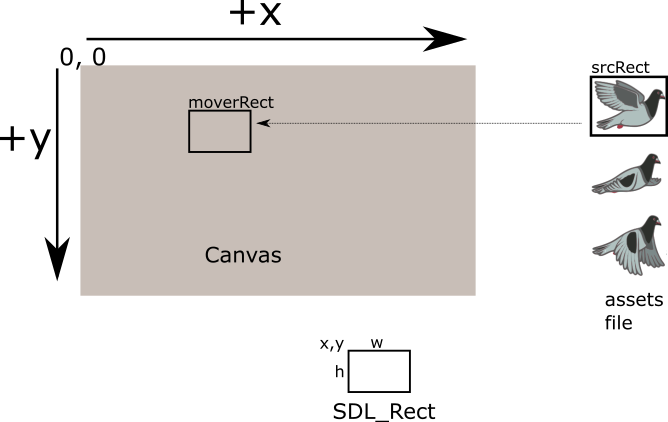
\includegraphics[width=\linewidth]{sdlDrawing}
		\caption{SDL Drawing Basics}
		\label{fig:sdlDrawing}
	\end{figure}
	
	\section{Some important points:} 
	
	\begin{itemize}
		\item Sample code is there for your benefit. If you are going to use it, understand how it works. 
		\item You do not need to follow the code given exactly. You can make changes where you see fit provided that it makes sense.
%		\item Implement Q1 prior to implementing Q2, it will help you to implement linked list.
%		\item Where necessary, declare your own functions inside classes. Make sure why you would keep a function as private or public.

		\item You need to define separate \path{*.hpp} and \path{*.cpp} files for all the classes.
		\item Exact x,y,w,h values for images in assets file can be found by \url{http://www.spritecow.com/}. 
		\item A tutorial for file I/O is given \url{http://www.cplusplus.com/doc/tutorial/files/}. 
		\item You should take \url{www.cplusplus.com} and \url{www.cppreference.com} as primary web source to search about C++
		\item You have to follow best OOP practices as discussed in lectures.
	\end{itemize}
		\section{Rubric}
	\begin{table}[h]
		\centering
		\begin{tabular}{llc}
			\toprule
			Warnings/Errors	& The code had no warnings/errors	& 1 \\
			Comments &	The code was properly commented	& 1 \\
			Coding	& The code followed best practices guideline &	1 \\
			OOP Concepts & The code followed best OOP practices & 2 \\
			% Modularization &	Code is modularized in different functions	& 1\\
			Logic	& Logic is fully implemented	& 10 \\
			\midrule
			Total & & 15\\
			\bottomrule
		\end{tabular}
		\caption{Grading Rubric}
		\label{Grading}
	\end{table}
	\section{Credits}
		Some questions in this assignment are derived from the work of Dr. Umair Azfar Khan.
	\begin{center}
		-- The End --
	\end{center}
	\newpage
	
	
\end{document}